\section{覆叠变换}
\label{ch13-sec81}

对于给定的覆叠映射 $p\colon E\to B$, 考虑这个覆叠空间到其自身的所有等价所构成的集合是一个颇有意思的问题. 这样一个等价称为\textbf{覆叠变换}(covering transformation). 覆叠变换的复合、覆叠变换的逆都是覆叠变换, 所以覆叠变换构成的集合是一个群, 我们将其称为\textbf{覆叠变换群}(group of covering transformations), 记作 $\mathcal{C}(E,\ p,\ B)$.

本节始终假设 $p\colon E\to B$ 是一个覆叠映射, $p(e_{0})=b_{0}$, $H_{0}=p_{*}(\pi_{1}(E,\ e_{0}))$. 我们将证明 $\mathcal{C}(E,\ p,\ B)$ 完全被 $\pi_{1}(B,\ b_{0})$ 及其子群 $H_{0}$ 所确定. 特别地, 我们将证明: 如果 $N(H_{0})$ 是以 $H_{0}$ 为其正规子群的 $\pi_{1}(B,\ b_{0})$ 中最大的子群, 则 $\mathcal{C}(E,\ p,\ B)$ 同构于 $N(H_{0})/H_{0}$.

下面给出 $N(H_{0})$ 的正式定义.

\begin{definition}[正规化子]
\label{definition:ch13-normalizer}
若 $H$ 是群 $G$ 的一个子群, $H$ 在 $G$ 中的\textbf{正规化子}(normalizer)是指由以下等式给出的 $G$ 的子集:
\[
N(H)=\{g\mid gHg^{-1}=H\}.
\]
易见, $N(H)$ 是 $G$ 的一个子群. 根据定义, $N(H)$ 包含 $H$ 并且 $H$ 是它的正规子群, $N(H)$ 也是 $G$ 中以 $H$ 为正规子群的最大子群.
\end{definition}

应用第 54 节中的提升对应以及第 79 节中证明的关于等价的存在的结论来建立 $N(H_{0})/H_{0}$ 与 $\mathcal{C}(E,\ p,\ B)$ 之间的对应. 首先给出以下定义.

给定 $p\colon E\to B$, $p(e_{0})=b_{0}$. 设 $F$ 为集合 $F=p^{-1}(e_{0})$. 设
\[
\Phi\colon\pi_{1}(B,b_{0})/H_{0}\longrightarrow F
\]
为定理 54.6 中给出的提升对应, 它是一个一一映射. 此外定义以下对应:
\[
\Psi\colon\mathcal{C}(E,p,B)\longrightarrow F
\]
使得对于每一个覆叠变换 $h\colon E\to E$, $\Psi(h)=h(e_{0})$. 由于 $h$ 被它在 $e_{0}$ 处的值所唯一地决定, 因此 $\Psi$ 是一个单射.

\begin{lemma}[$\Psi$ 的像]
\label{lemma:ch13-psi-image}
映射 $\Psi$ 的像等于 $\pi_{1}(B,\ b_{0})/H_{0}$ 的子群 $N(H_{0})/H_{0}$ 在 $\Phi$ 下的像.
\end{lemma}

\begin{proof}
提升对应 $\phi\colon\pi_{1}(B,\ b_{0})\to F$ 是按以下方式定义的: 给定 $B$ 中以 $b_{0}$ 为基点的一条回路 $\alpha$, 设 $E$ 中以 $e_{0}$ 为基点的道路 $\gamma$ 是它的提升, 令 $e_{1}=\gamma(1)$, $\phi$ 定义为 $\phi([\alpha])=e_{1}$. 为了证明本引理, 需要证明存在一个满足条件 $h(e_{0})=e_{1}$ 的覆叠变换 $h\colon E\to E$ 当且仅当 $[\alpha]\in N(H_{0})$.

证明这一点是容易的. \cref{lemma:ch13-conjugate-fibers} 告诉我们: $h$ 存在当且仅当 $H_{0}=H_{1}$, 其中 $H_{1}=p_{*}(\pi_{1}(E,\ e_{1}))$. 而该引理告诉我们: $[\alpha]*H_{1}*[\alpha]^{-1}=H_{0}$. 因此 $h$ 存在当且仅当 $[\alpha]*H_{0}*[\alpha]^{-1}=H_{0}$, 这等于说 $[\alpha]\in N(H_{0})$.
\end{proof}

\begin{theorem}[覆叠变换群同构于 $N(H_{0})/H_{0}$]
\label{theorem:ch13-covering-group-isomorphism}
一一映射
\[
\Phi^{-1}\circ\Psi\colon\mathcal{C}(E,p,B)\longrightarrow N(H_{0})/H_{0}
\]
是两个群之间的一个同构.
\end{theorem}

\par
\begin{figure}[htbp]
\centering
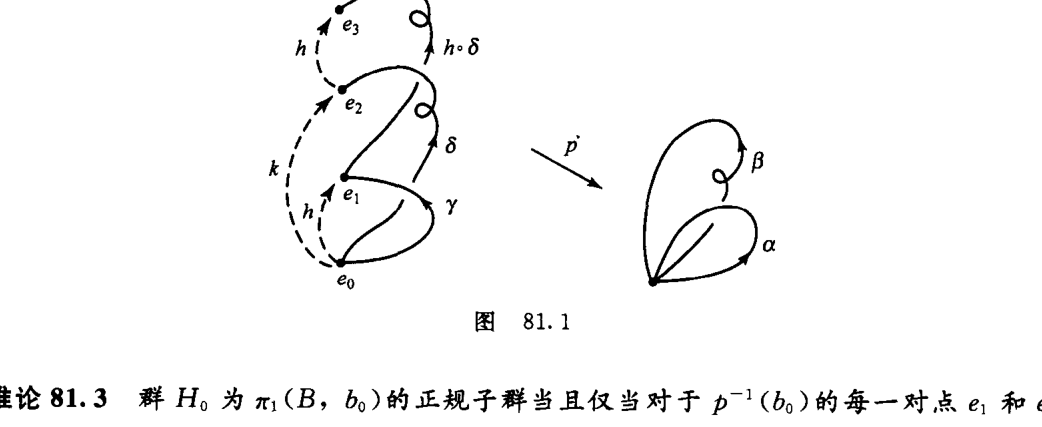
\includegraphics[width=0.7\textwidth]{image/fig-81-1.png}
\caption{覆叠变换的复合在覆叠纤维上的作用.}
\label{ch13-fig-81-1}
\end{figure}

\begin{proof}
我们仅需证明 $\Phi^{-1}\circ\Psi$ 是一个同态. 设 $h$, $k\colon E\to E$ 是两个覆叠变换. 令 $h(e_{0})=e_{1}$ 和 $k(e_{0})=e_{2}$. 根据定义, 有
\[
\Psi(h)=e_{1}\qquad\text{和}\qquad\Psi(k)=e_{2}.
\]
分别选取 $E$ 中从 $e_{0}$ 到 $e_{1}$ 和 $e_{2}$ 的道路 $\gamma$ 和 $\delta$. 若 $\alpha=p\circ\gamma$ 和 $\beta=p\circ\delta$, 则根据定义有
\[
\Phi([\alpha]H_{0})=e_{1}\qquad\text{和}\qquad\Phi([\beta]H_{0})=e_{2}.
\]
设 $e_{3}=h(k(e_{0}))$, 则有 $\Psi(h\circ k)=e_{3}$. 为了证明定理, 我们只需证明
\[
\Phi([\alpha*\beta]H_{0})=e_{3}.
\]
由于 $\delta$ 是从 $e_{0}$ 到 $e_{2}$ 的道路, 所以 $h\circ\delta$ 是从 $h(e_{0})=e_{1}$ 到 $h(e_{2})=h(k(e_{0}))=e_{3}$ 的道路. 参见\cref{ch13-fig-81-1}. 这时乘积 $\gamma*(h\circ\delta)$ 有定义并且是一条从 $e_{0}$ 到 $e_{3}$ 的道路. 这条道路是 $\alpha*\beta$ 的一个提升, 这是由于 $p\circ\gamma=\alpha$ 和 $p\circ h\circ\delta=p\circ\delta=\beta$. 因此, $\Phi([\alpha*\beta]H_{0})=e_{3}$, 这便是我们所要证明的.

\end{proof}

\begin{corollary}[正规子群与齐性覆叠]
\label{corollary:ch13-regular-homogeneous}
群 $H_{0}$ 为 $\pi_{1}(B,\ b_{0})$ 的正规子群当且仅当对于 $p^{-1}(b_{0})$ 的每一对点 $e_{1}$ 和 $e_{2}$, 存在一个覆叠变换 $h\colon E\to E$ 使得 $h(e_{1})=e_{2}$. 这时, 存在一个同构
\[
\Phi^{-1}\circ\Psi\colon\mathcal{C}(E,p,B)\longrightarrow\pi_{1}(B,b_{0})/H_{0}.
\]
\end{corollary}

\begin{corollary}[万有覆叠的变换群]
\label{corollary:ch13-universal-transform-group}
设 $p\colon E\to B$ 为覆叠映射. 如果 $E$ 是单连通的, 则
\[
\mathcal{C}(E,p,B)\cong\pi_{1}(B,b_{0}).
\]
\end{corollary}

若 $H_{0}$ 是 $\pi_{1}(B,\ b_{0})$ 的一个正规子群, 则 $p\colon E\to B$ 称为\textbf{正则覆叠映射}(regular covering map). (请注意不要弄混淆, "正规"和"正则", 这两个术语已被赋予了完全不同的含义!)

\begin{example}[圆周的覆叠变换群]
\label{example:ch13-circle-transform}
由于圆周的基本群是一个阿贝尔群, $S^{1}$ 的每一个覆叠映射都是正则的. 如果 $p\colon\mathbb{R}\to S^{1}$ 是标准覆叠映射, 则覆叠变换便是同胚 $x\mapsto x+n$. 因此相应的覆叠变换群同构于 $\mathbb{Z}$.
\end{example}

\par
\begin{figure}[htbp]
\centering
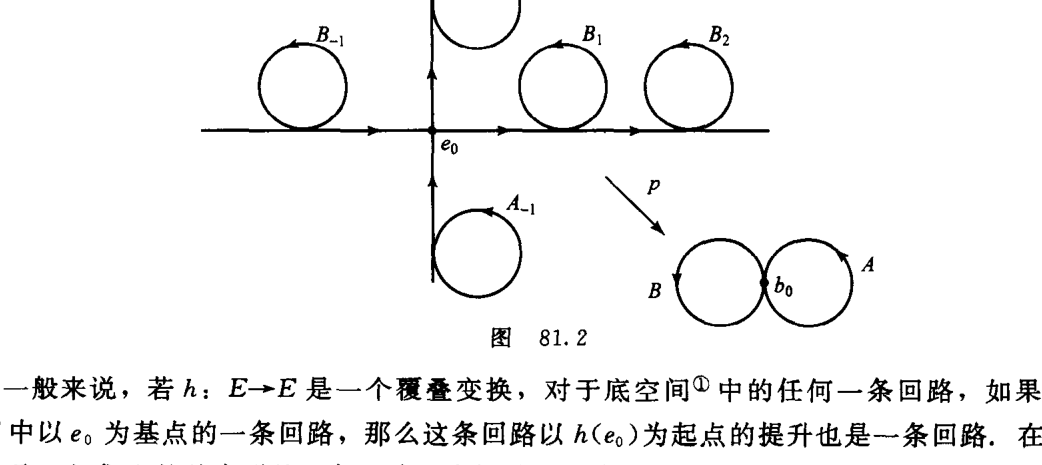
\includegraphics[width=0.85\textwidth]{image/fig-81-2.png}
\caption{$8$ 字形空间的一个覆叠空间.}
\label{ch13-fig-81-2}
\end{figure}

\begin{example}[8 字形空间覆叠的平凡变换群]
\label{example:ch13-figure-eight-trivial}
作为另一个极端的例子, 我们考虑如\cref{ch13-fig-81-2} 所示的 $8$ 字形空间的覆叠空间. (在第 60 节中我们曾考虑过这个覆叠空间: 将 $x$ 轴缠绕到圆周 $A$ 上, $y$ 轴缠绕到圆周 $B$ 上. 圆周 $A_{i}$ 和圆周 $B_{i}$ 分别被同胚地映射到 $A$ 和 $B$ 上.) 我们将证明群 $\mathcal{C}(E,\ p,\ B)$ 为平凡群.


一般来说, 若 $h\colon E\to E$ 是一个覆叠变换, 对于底空间中的任何一条回路, 如果可提升为 $E$ 中以 $e_{0}$ 为基点的一条回路, 那么这条回路以 $h(e_{0})$ 为起点的提升也是一条回路. 在当前的情形下, 生成 $A$ 的基本群的一条回路, 当提升的起点取为 $e_{0}$ 时, 它的提升不是一条回路, 而当提升的起点取为 $p^{-1}(b_{0})$ 中位于 $y$ 轴上的其他点时, 它的提升才是一条回路. 类似地, 生成 $B$ 的基本群的一条回路, 当提升的起点取为 $e_{0}$ 时, 它的提升不是一条回路, 而当提升的起点取为 $p^{-1}(b_{0})$ 中位于 $x$ 轴上的其他点时, 它的提升才是一条回路. 由此可见, $h(e_{0})=e_{0}$, 从而 $h$ 是恒等映射.
\end{example}

有这样一种直接构造正则的覆叠空间的办法, 事实上, 每一个正则的覆叠空间都可以通过这种方式来构造. 这涉及一个群在空间上的作用.

\begin{definition}[轨道空间与纯不连续作用]
\label{definition:ch13-orbit-space}
设 $X$ 是一个空间, $G$ 是从 $X$ 到自身的同胚群的一个子群. \textbf{轨道空间}(orbit space) $X/G$ 是 $X$ 相对于下述等价关系的商空间: 对任意 $x\in X$ 和任意 $g\in G$ 定义 $x\sim g(x)$. $x$ 的等价类称为 $x$ 的\textbf{轨道}(orbit).

若 $G$ 是空间 $X$ 的所有同胚所构成的群, $G$ 在 $X$ 上的作用称为是\textbf{纯不连续的}(properly discontinuous), 如果对于每一个 $x\in X$ 都存在 $x$ 的一个邻域 $U$, 使得 $g(U)$ 与 $U$ 无交. ($g\neq e$, $e$ 为 $G$ 的单位元.) 因此, 当 $g_{0}\neq g_{1}$ 时便有 $g_{0}(U)$ 与 $g_{1}(U)$ 无交, 否则 $U$ 与 $g_{0}^{-1}g_{1}(U)$ 将不是无交的.
\end{definition}

\begin{theorem}[纯不连续作用给出正则覆叠]
\label{theorem:ch13-properly-discontinuous}
设 $X$ 是道路连通且局部道路连通的, $G$ 为由 $X$ 上的所有同胚构成的群. 则商映射 $\pi\colon X\to X/G$ 是一个覆叠映射当且仅当 $G$ 的作用是纯不连续的. 此时, 覆叠映射 $\pi$ 是正则的并且 $G$ 是覆叠变换群.
\end{theorem}

\begin{proof}
首先证明 $\pi$ 是一个开映射. 若 $U$ 为 $X$ 中的开集, 则 $\pi^{-1}\pi(U)$ 是 $X$ 中形如 $g(U)$ 的开集的并, 其中 $g$ 取遍 $G$ 的所有元素. 因此 $\pi^{-1}\pi(U)$ 为 $X$ 中的开集, 根据定义, $\pi(U)$ 是 $X/G$ 中的开集. 因此 $\pi$ 是开的.

\textbf{第一步.} 假设 $G$ 的作用是纯不连续的, 我们来证明 $\pi$ 是一个覆叠映射. 给定 $x\in X$, 设 $U$ 是 $x$ 的一个邻域, 使得当 $g_{0}\neq g_{1}$ 时 $g_{0}(U)$ 与 $g_{1}(U)$ 无交. 则 $\pi$ 均衡地覆盖着 $\pi(U)$. 事实上, $\pi^{-1}\pi(U)$ 等于那些无交开集 $g(U)$ 的并, 其中 $g$ 取遍 $G$, 并且每一个 $g(U)$ 最多包含每一条轨道的一个点. 因此, 由限制 $\pi$ 所得到的映射 $g(U)\to\pi(U)$ 作为连续开映射, 是一个一一映射, 因此是一个同胚. 因此当 $g$ 取遍 $G$ 时所有集合 $g(U)$ 形成 $\pi^{-1}\pi(U)$ 的一个片状分拆.

\textbf{第二步.} 假设 $\pi$ 是一个覆叠映射, 我们来证明 $G$ 的作用是纯不连续的. 给定 $x\in X$, 设 $V$ 是 $\pi(x)$ 的一个被 $\pi$ 均衡地覆盖着的邻域. 考虑 $\pi^{-1}(V)$ 的片状分拆, 设 $U_{\alpha}$ 为其中含有 $x$ 的那一片. 任意给定 $g\in G$, $g\neq e$, 则 $g(U_{\alpha})$ 必定与 $U_{\alpha}$ 无交, 否则将会有 $U_{\alpha}$ 中的两个点在同一条轨道中, 这将导致 $\pi$ 限制于 $U_{\alpha}$ 不是单射. 因此 $G$ 的作用是纯不连续的.

\textbf{第三步.} 若 $\pi$ 是一个覆叠映射, 我们来证明 $G$ 是覆叠变换群且 $\pi$ 是正则的. 显然, 当 $\pi\circ g=\pi$ 时, 任何 $g\in G$ 都是覆叠变换, 这是由于 $g(x)$ 的轨道等于 $x$ 的轨道. 另一方面, 设 $h$ 是一个满足条件 $h(x_{1})=x_{2}$ 的覆叠变换. 因为 $\pi\circ h=\pi$, 从而点 $x_{1}$ 和 $x_{2}$ 在映射 $\pi$ 下有相同的像, 因此存在一个元素 $g\in G$, 使得 $g(x_{1})=x_{2}$. 定理 79.2 中的唯一性部分蕴涵着 $h=g$.

由此可见 $\pi$ 是正则的. 事实上, 对于同一轨道中的任何两个点 $x_{1}$ 和 $x_{2}$, 存在一个元素 $g\in G$ 使得 $g(x_{1})=x_{2}$. 再应用 \cref{corollary:ch13-regular-homogeneous} 便可得到所要的结论.
\end{proof}

\begin{theorem}[正则覆叠空间的轨道表示]
\label{theorem:ch13-regular-orbit}
若 $p\colon X\to B$ 是一个正则的覆叠映射, $G$ 是 $p$ 的覆叠变换群, 则存在一个同胚 $k\colon X/G\to B$ 使得 $p=k\circ\pi$, 其中 $\pi\colon X\to X/G$ 为投射.
\end{theorem}

\begin{proof}
若 $g$ 是一个覆叠变换, 则根据定义有 $p(g(x))=p(x)$. 因此在每一轨道上 $p$ 为常值映射, 从而它诱导出从商空间 $X/G$ 到 $B$ 的一个连续映射 $k$. 另一方面, 因为 $p$ 是一个满的连续开映射, 所以 $p$ 是一个商映射. 由于 $p$ 是正则的, 在 $G$ 的作用下 $p^{-1}(b)$ 中的任何两点属于同一轨道. 因此, $\pi$ 诱导出一个连续映射 $B\to X/G$, 它是 $k$ 的逆映射.
\end{proof}

\par
\begin{figure}[htbp]
\centering
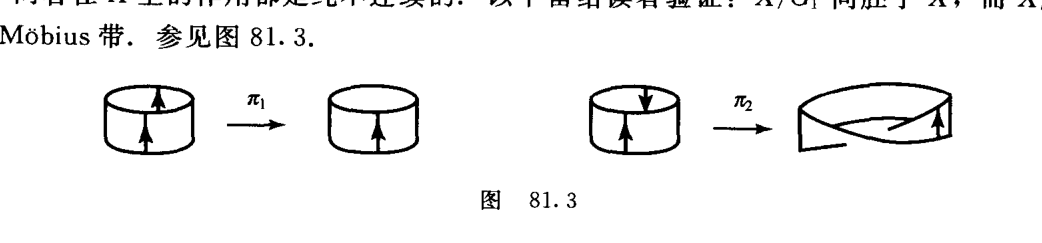
\includegraphics[width=0.85\textwidth]{image/fig-81-3.png}
\caption{柱面分别经 $G_{1}$ 与 $G_{2}$ 作用所得的轨道空间.}
\label{ch13-fig-81-3}
\end{figure}

\begin{example}[柱面与 Möbius 带]
\label{example:ch13-cylinder-mobius}
设 $X$ 是圆柱面 $S^{1}\times I$. $h\colon X\to X$ 是一个同胚, 其中 $h(x,\ t)=(-x,\ t)$. $k\colon X\to X$ 也是一个同胚, 定义为 $k(x,\ t)=(-x,\ 1-t)$. 群 $G_{1}=\{e,\ h\}$ 和 $G_{2}=\{e,\ k\}$ 都同构于整数模 $2$ 群, 两者在 $X$ 上的作用都是纯不连续的. 以下留给读者验证: $X/G_{1}$ 同胚于 $X$, 而 $X/G_{2}$ 同胚于 Möbius 带. 参见\cref{ch13-fig-81-3}.

\end{example}

\begin{exercise}
\label{exercise:ch13-sec81-01}
\begin{enumerate}[(a)]
\item 给出一个 $2$ 阶的环面 $T$ 的同胚群 $G$, 使得 $T/G$ 同胚于环面.
\item 给出一个 $2$ 阶的环面 $T$ 的同胚群 $G$, 使得 $T/G$ 同胚于 Klein 瓶.
\end{enumerate}
\end{exercise}

\par
\begin{figure}[htbp]
\centering
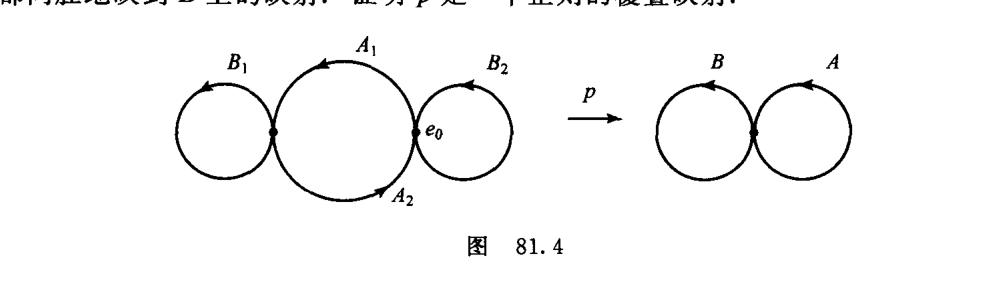
\includegraphics[width=0.8\textwidth]{image/fig-81-4.png}
\end{figure}

\par
\begin{figure}[htbp]
\centering
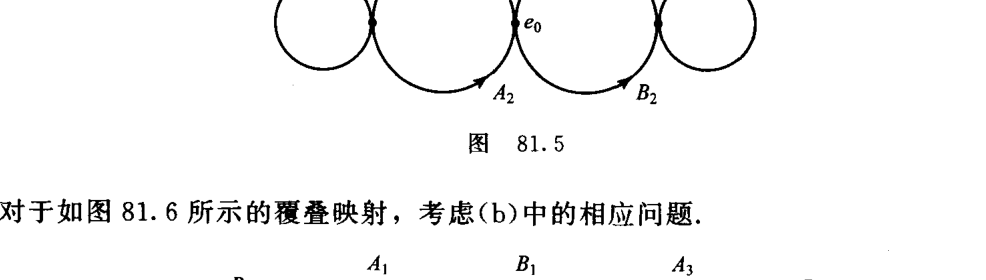
\includegraphics[width=0.8\textwidth]{image/fig-81-5.png}
\end{figure}

\par
\begin{figure}[htbp]
\centering
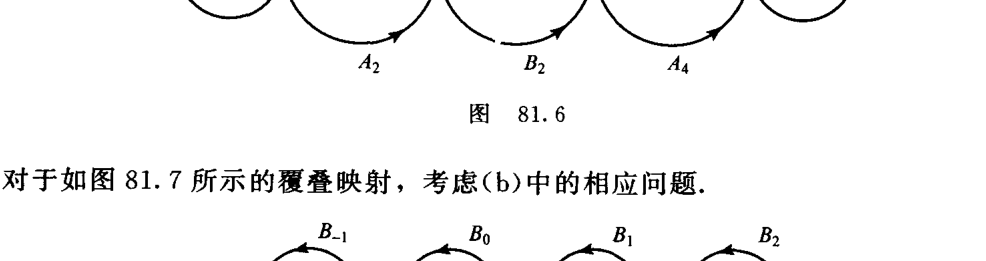
\includegraphics[width=0.8\textwidth]{image/fig-81-6.png}
\end{figure}

\par
\begin{figure}[htbp]
\centering
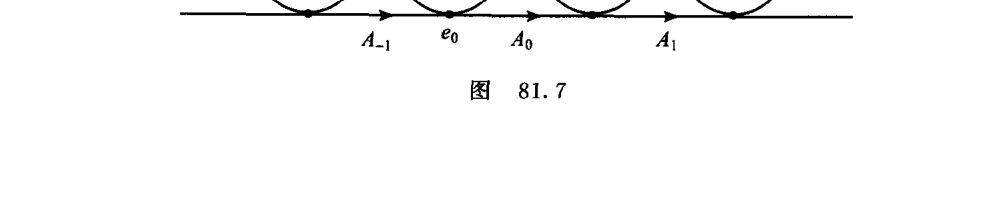
\includegraphics[width=0.85\textwidth]{image/fig-81-7.png}
\end{figure}

\begin{exercise}
\label{exercise:ch13-sec81-02}
设 $X=A\vee B$ 是两个圆周的束.
\begin{enumerate}[(a)]
\item 设 $E$ 是画在\cref{ch13-fig-81-4} 中的空间, $p\colon E\to X$ 表示将弧 $A_{1}$ 和弧 $A_{2}$ 都缠绕 $A$ 并且将 $B_{1}$ 和 $B_{2}$ 都同胚地映到 $B$ 上的映射. 证明 $p$ 是一个正则的覆叠映射.
\item 试确定如\cref{ch13-fig-81-5} 所示的 $X$ 的覆叠空间的覆叠变换群. 这个覆叠映射是否是正则的?
\item 对于如\cref{ch13-fig-81-6} 所示的覆叠映射, 考虑 (b) 中的相应问题.
\item 对于如\cref{ch13-fig-81-7} 所示的覆叠映射, 考虑 (b) 中的相应问题.
\end{enumerate}
\end{exercise}

\begin{exercise}
\label{exercise:ch13-sec81-03}
设 $p\colon X\to B$ 是覆叠映射 (不必是正则的), $G$ 为 $p$ 的覆叠变换群.
\begin{enumerate}[(a)]
\item 证明 $G$ 在 $X$ 上的作用是纯不连续的.
\item 设 $\pi\colon X\to X/G$ 是投射. 证明存在一个覆叠映射 $k\colon X/G\to B$ 使得 $k\circ\pi=p$.
\end{enumerate}
\end{exercise}

\begin{exercise}
\label{exercise:ch13-sec81-04}
设 $G$ 是 $X$ 的一个同胚群. $G$ 在 $X$ 上的作用称为是\textbf{不动点平凡的}(fixed-point free)的, 如果除恒等映射 $e$ 外 $G$ 中的任何成员都没有不动点. 证明: 若 $X$ 是一个 Hausdorff 空间, 且 $G$ 是 $X$ 的不动点平凡的有限同胚群, 则 $G$ 的作用是纯不连续的.
\end{exercise}

\begin{exercise}
\label{exercise:ch13-sec81-05}
将 $S^{3}$ 视为满足条件 $|z_{1}|^{2}+|z_{2}|^{2}=1$ 的所有复数点偶 $(z_{1},\ z_{2})$ 构成的空间. 给定互素正整数 $n$ 和 $k$, 映射 $h\colon S^{3}\to S^{3}$ 定义为
\[
h(z_{1},z_{2})=(z_{1}e^{2\pi i/n},z_{2}e^{2\pi ik/n}).
\]
\begin{enumerate}[(a)]
\item 证明 $h$ 生成 $S^{3}$ 的同胚群的一个 $n$ 阶循环子群 $G$, 并且除 $G$ 的单位元以外其他元素没有不动点. 轨道空间 $S^{3}/G$ 称为\textbf{透镜空间}(lens space) $L(n,\ k)$.
\item 证明: 若 $L(n,\ k)$ 与 $L(n',\ k')$ 同胚, 则 $n=n'$. [有这样一个定理: $L(n,\ k)$ 与 $L(n',\ k')$ 同胚当且仅当 $n=n'$ 并且 $k\equiv k'(\bmod\ n)$ 或者 $kk'\equiv 1(\bmod\ n)$. 其证明绝对不平凡.]
\item 证明 $L(n,\ k)$ 是一个紧致 $3$-维流形.
\end{enumerate}
\end{exercise}

\begin{exercise}
\label{exercise:ch13-sec81-06}
\begin{theorem}[局部紧 Hausdorff 空间上的纯不连续作用]
设 $X$ 是一个局部紧的 Hausdorff 空间, $G$ 是 $X$ 的一个同胚群, 使得 $G$ 的作用是不动点平凡的. 假设对于 $X$ 的每一个紧致子空间 $C$, 仅有有限多个 $G$ 的元素 $g$ 使得交 $C\cap g(C)$ 非空. 则 $G$ 的作用是纯不连续的, 并且 $X/G$ 也是局部紧的 Hausdorff 空间.
\end{theorem}
\begin{enumerate}[(a)]
\item 对于 $X$ 的每一个紧致子空间 $C$, 证明对于所有的 $g\in G$, 集合 $g(C)$ 的并是 $X$ 中的闭集. [提示: 若 $U$ 是 $x$ 的一个邻域使得 $\overline{U}$ 紧致, 那么仅有有限多个 $g$ 使得 $\overline{U}\cup C$ 与 $g(\overline{U}\cup C)$ 有非空的交.]
\item 证明 $X/G$ 是一个 Hausdorff 空间.
\item 证明 $G$ 的作用是纯不连续的.
\item 证明 $X/G$ 是局部紧的.
\end{enumerate}
\end{exercise}
